 \newpage
 \section{Resultados}
 
 \subsection{HPO}
 Esta enfermedad, Trombosis Arterial, está definida como HPO:0004420, manteniendo relación con otras 26 enfermedades y con 25 genes asociados.
 
 \subsection{STRING}
 Con la base de datos biológica STRING, hemos obtenido los genes asociados y sus interacciones.
 
 \begin{minipage}{\linewidth}
 	\makebox[\linewidth]{
		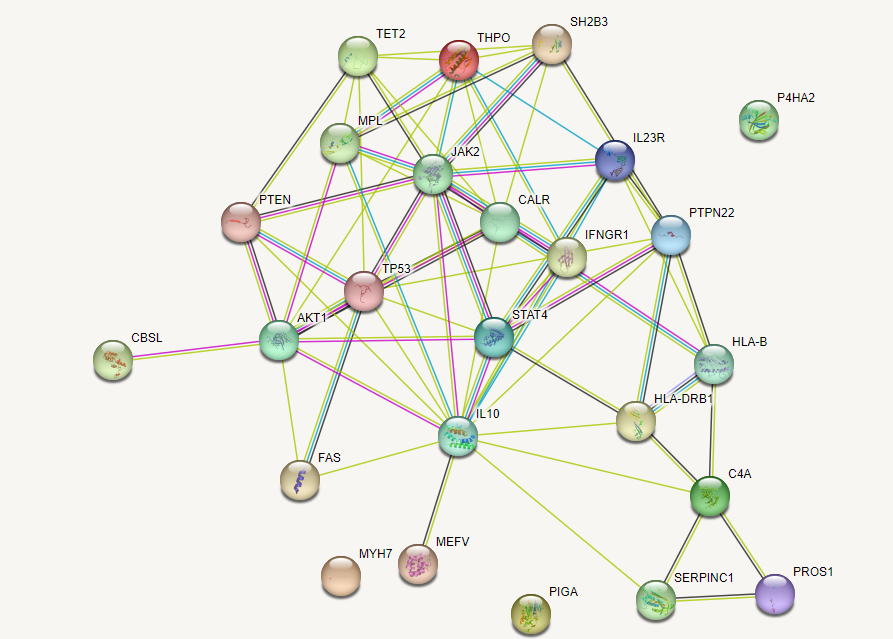
\includegraphics[width=0.70\textwidth]{figures/genes_asociados.png}

 	}
 	\captionof{figure}{Genes asociados a la trombosis.}
 	\label{fig: Figura 3}
 \end{minipage}



\subsection{Comunidades}
Con la propagación de genes en \textit{STRING} hemos obtenido el siguiente grafo de 70 genes (45 semillas).

 \begin{minipage}{\linewidth}
	\makebox[\linewidth]{
	 	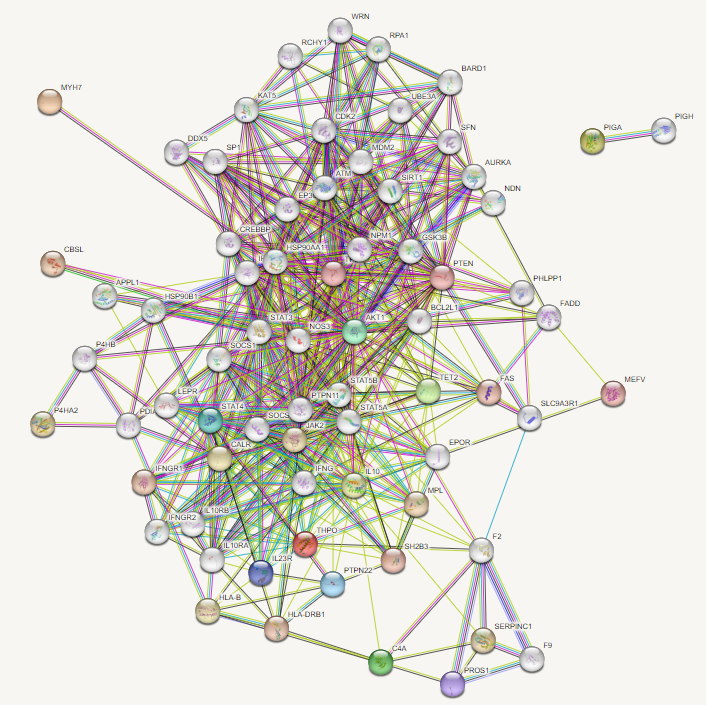
\includegraphics[width=0.70\textwidth]{figures/network_propagation.png}
		
	}
	\captionof{figure}{Conjunto de genes tras la propagación, siendo los de color gris genes semilla y los de color los iniciales representados en la figura \ref{fig: Figura 3}.}
	\label{fig: Figura 4}
\end{minipage}

\begin{spacing}{1}
Se han obtenido un total de 18 comunidades genéticas, con el paquete \textit{linkcomm}, representadas en la figura 5. Vemos que la comunidad morada es la comunidad más amplia. 
\end{spacing}

\begin{minipage}{\linewidth}
	\makebox[\linewidth]{
		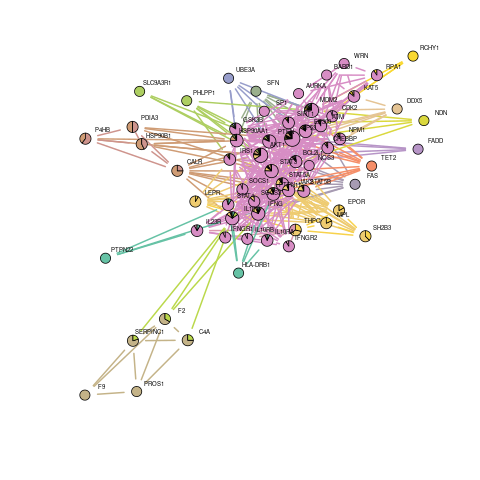
\includegraphics[width=0.70\textwidth]{figures/01_NetworkComunidades.png}
		
	}
	\captionof{figure}{Comunidades genéticas generadas con el paquete \textit{linkcomm} al conjunto de genes representados en la figura  \ref{fig: Figura 4}.}
	\label{fig: Figura 5}
\end{minipage}

\begin{spacing}{1}
También, en la figura \ref{fig: Figura6}, vemos las comunidades independientes de nuestro reactoma. En nuestro caso, las comunidades independientes son dos y estarían conformadas por un lado por \textit{P4HB, PDIA3, CALR, HSP90B1} y por otro lado por \textit{LEPR, THPO, MPL, SH2B3, EPOR}
\end{spacing}

\begin{minipage}{\linewidth}
	\makebox[\linewidth]{
		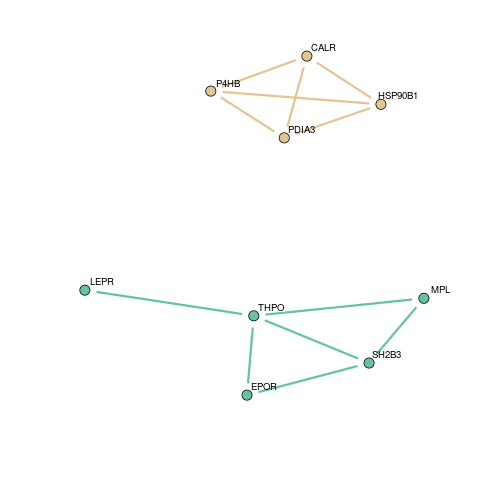
\includegraphics[width=0.70\textwidth]{figures/05_Comunidades_Independientes.png}
		
	}
	\captionof{figure}{Comunidades genéticas independientes generadas con el paquete \textit{linkcomm} al conjunto de genes representados en la figura  \ref{fig: Figura 5}.}
	\label{fig: Figura6}
\end{minipage}


\begin{spacing}{1}
	En la figura \ref{fig: Figura 7} podemos ver una matriz con los genes que unen y, por tanto, pertenecen a más comunidades. En nuestro caso, podemos observar que los genes TP53 y AKT1 son los genes que unen y pertenecen a más comunidades con 10 y 8 conexiones respectivamente, marcado a la derecha. En la parte posterior del gráfico nos indica las comunidades a las que pertenecen estos genes, colocándose en la parte inferior la sumatoria de las comunidades a las que pertenecen estos diez genes. Vemos, que todos son parte de la comunidad 16.
\end{spacing}



\begin{minipage}{\linewidth}
	\makebox[\linewidth]{
		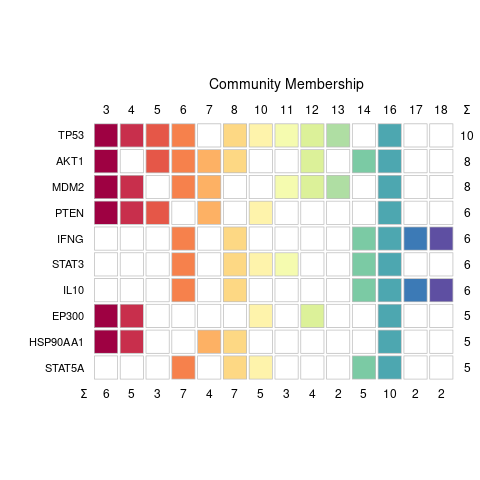
\includegraphics[width=0.70\textwidth]{figures/03_GenesMasCOnectadosOtrasComunidades.png}
		
	}
	\captionof{figure}{Matriz de genes por comunidad}
	\label{fig: Figura 7}
\end{minipage}


En la figura \ref{fig: Figura 8} podemos ver los genes con mayor centralidad

\begin{minipage}{\linewidth}
	\makebox[\linewidth]{
		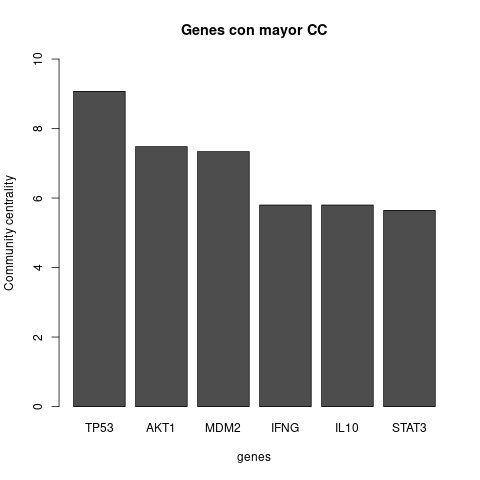
\includegraphics[width=0.70\textwidth]{figures/04_GenesMayorCentralidad.png}
		
	}
	\captionof{figure}{Genes con mayor centralidad}
	\label{fig: Figura 8}
\end{minipage}



\subsection{Enriquecimiento de las comunidades}
Se ha realizado el enriquecimiento a todas las comunidades, los ficheros .csv se pueden visualizar en el GitHub en la carpeta 'results'.

